\documentclass{article}
\usepackage[utf8]{inputenc}
\usepackage{braket}
\usepackage{amsmath}
\usepackage{graphicx}
\usepackage{float}
\usepackage{hyperref}
\usepackage{caption}
\usepackage{subcaption}
\usepackage{derivative}

\usepackage{geometry}
\geometry{
    a4paper,
    total={170mm,257mm},
    left=20mm,
    top=20mm,
}

\graphicspath{ {../plots} }

\title{Simulating reaction of Ne* + OCS collision}
\author{Marcin Welter}
\date{Winter semester 2024/2025}

\newcommand{\centered}[1]{\begin{tabular}{l} #1 \end{tabular}}
\newcommand{\cmg}{\frac{\text{cm}^3}{\text{s}}}
\newcommand{\ak}{\hspace{50pt}}

\newcommand{\doubleImage}[2]{
    \begin{figure}[H]
        \centering
        \begin{subfigure}{.49\linewidth}
            \centering
            \includegraphics[width=\linewidth]{#1}
        \end{subfigure}
        \begin{subfigure}{.49\linewidth}
            \centering
            \includegraphics[width=\linewidth]{#2}
        \end{subfigure}
    \end{figure}
}

\newcommand{\doubleImageCaption}[5]{
    \begin{figure}[H]
        \centering
        \begin{subfigure}{.49\linewidth}
            \centering
            \includegraphics[width=\linewidth]{#1}
            \caption{#2}
        \end{subfigure}
        \begin{subfigure}{.49\linewidth}
            \centering
            \includegraphics[width=\linewidth]{#3}
            \caption{#4}
        \end{subfigure}
        \caption{#5}
    \end{figure}
}

\begin{document}
\maketitle

\section{Improved potential interpolations}
    Potential is now fitted to the force field instead of interpolation, because of smoothness issues.
    Gamma potentials now have correct vanishing derivatives for angles $0$ and $\pi$.

    \doubleImageCaption{potential.pdf}{Data}{potential_interp.pdf}{Fitted}{Fitting of intermolecular potential}
    
    \doubleImageCaption{xpi_gamma.pdf}{Data}{xpi_gamma_interp.pdf}{Interpolated}{Interpolation of $X\Pi$ gamma potential}
    
    \doubleImageCaption{bsigma_gamma.pdf}{Data}{bsigma_gamma_interp.pdf}{Interpolated}{Interpolation of $B\Sigma$ gamma potential}

    \doubleImageCaption{api_gamma.pdf}{Data}{api_gamma_interp.pdf}{Interpolated}{Interpolation of $A\Pi$ gamma potential}

\section{Reaction rate ratio dependence on scaling force field parameters}
    Scaling the parameters of the force field (fitted as well as with theoretical values)
    did not change significantly the reaction rate ratio between different initial j from value of 1.
    As an example we show carbon attraction strength scaling of fitted force field.

    \begin{figure}[H]
        \centering
        \begin{subfigure}{.4\linewidth}
            \centering
            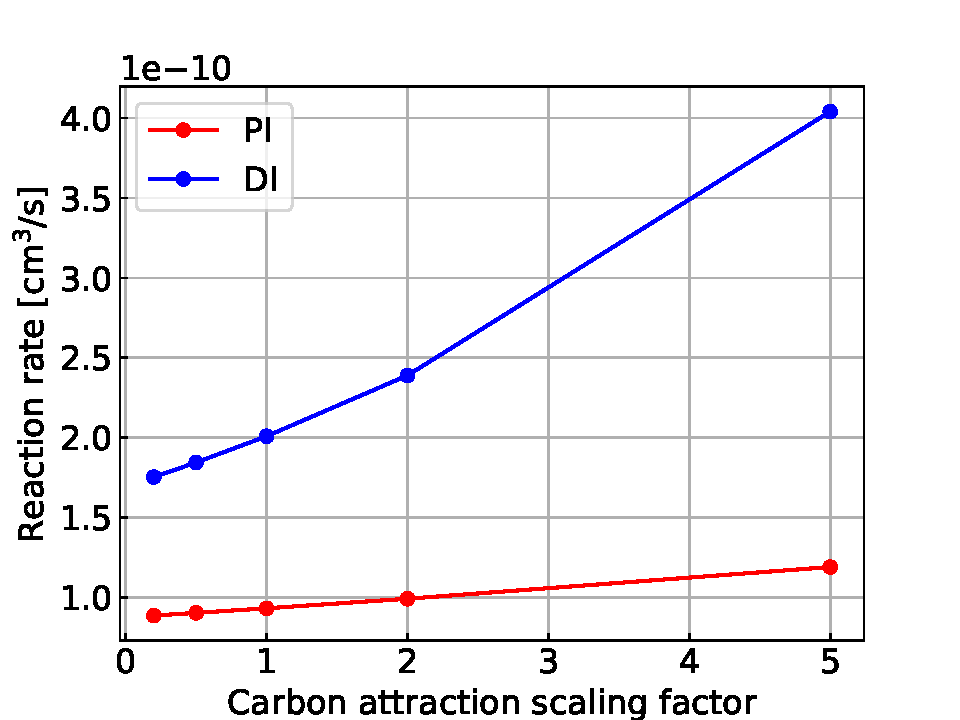
\includegraphics[width=\linewidth]{attr_c_scaling_0.pdf}
            \caption{Reaction rate for $j = 0$.}
        \end{subfigure}
        \begin{subfigure}{.4\linewidth}
            \centering
            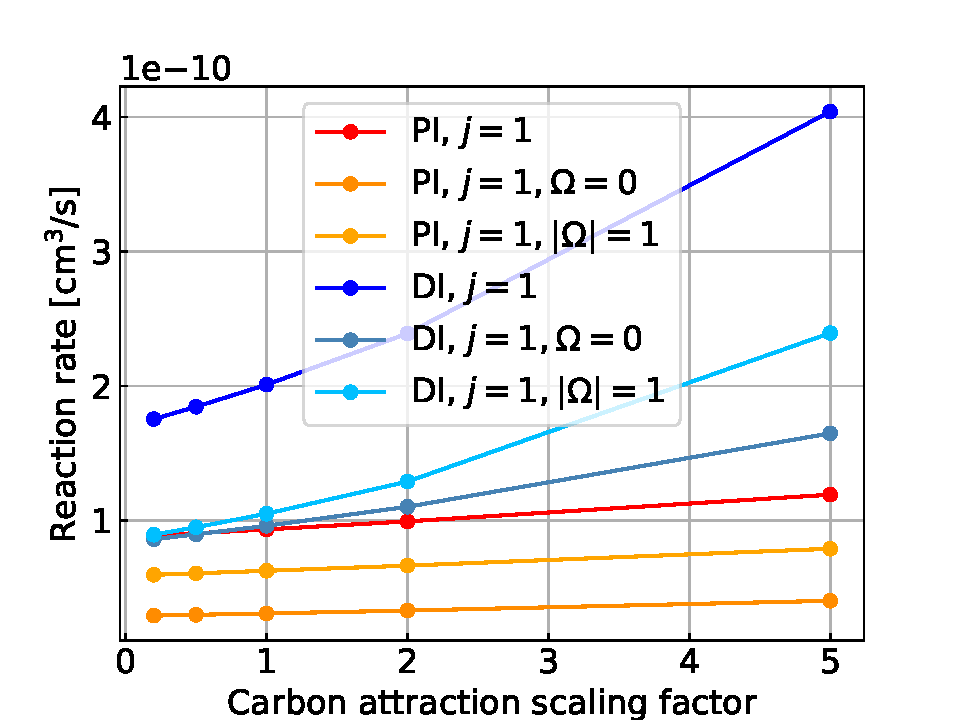
\includegraphics[width=\linewidth]{attr_c_scaling_1.pdf}
            \caption{Reaction rate for $j = 1$.}
        \end{subfigure}     
        \caption{Calculated reaction rates dependence on carbon attraction strength.}
    \end{figure}

    \begin{figure}[H]
        \centering
        \begin{subfigure}{.7\linewidth}
            \centering
            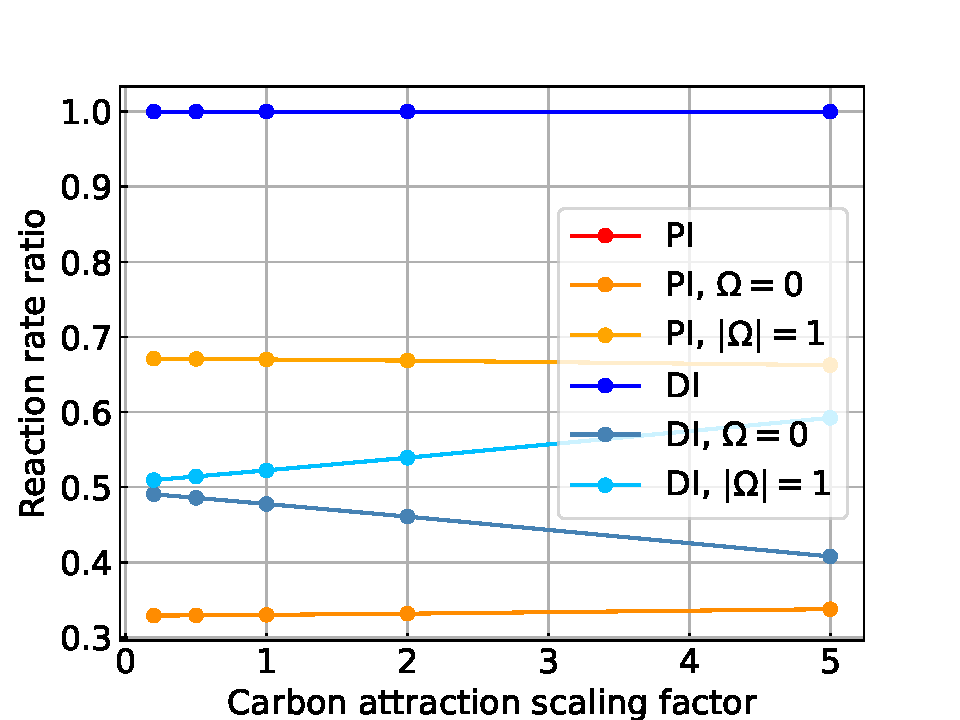
\includegraphics[width=\linewidth]{attr_c_scaling_ratio.pdf}
        \end{subfigure} 
        \caption{Calculated reaction rate ratio between $j = 1$ and $j = 0$, dependence on carbon attraction strength.}
    \end{figure}


\section{Truth tests for coriolis effect inclusion}
    To test coriolis effect inclusion, we compare the ground state energy 
    of the modified harmonic oscillator using different reference frames.

    The system defined by the space-fixed Hamiltonian is
    \begin{equation}
        \hat{H} = -\frac{1}{2\mu} \pdv*[order=2]{}{R} + \frac{\hat{L}^2}{2 \mu R^2} + V(R, \theta),
    \end{equation}
    this frame is equivalent to the body-fixed frame that we use for calculations, with rotational constant $B = 0$,
    the Hamiltonian is
    \begin{equation}
        \hat{H} = -\frac{1}{2\mu} \pdv*[order=2]{}{R} + \frac{(\hat{J} - \hat{j})^2}{2 \mu R^2} + V(R, \theta).
    \end{equation}

    The conserved quantities for the first system is the angular momentum projection number $m_l$,
    in case of the body-fixed frame the conserved quantity is the total angular momentum $J$.

    We use following harmonic oscillator potential
    \begin{equation}
        V(r, \theta) = \frac{\mu \omega^2}{2} (r - r_0)^2.
    \end{equation}

    The calculated ground state energy of the space-fixed Hamiltonian is equal to $\omega$ for projection $m_l = 0$.
    For the body-fixed Hamiltonian the calculated ground state for $J = 2$ is also $\omega$ with 
    coriolis effect and $1.08\omega$ if we neglect the coriolis effect and set $\Omega_\text{init} = 0$.
    Calculated wave-functions of the calculated ground state with and without coriolis effect are shown below.

    \begin{figure}[H]
        \centering
        \begin{subfigure}{.4\linewidth}
            \centering
            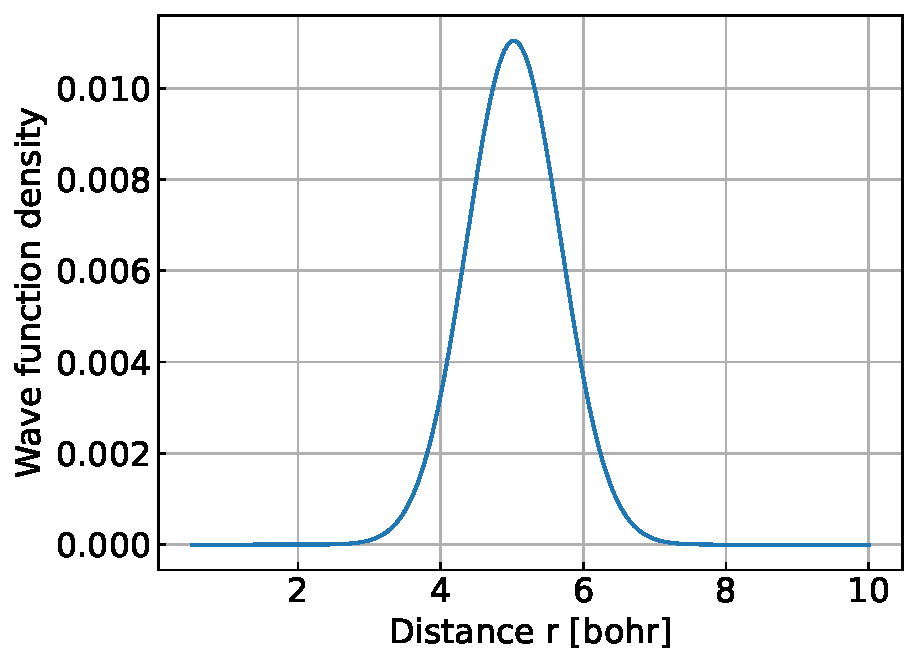
\includegraphics[width=\linewidth]{harmonic_iso_distance.pdf}
        \end{subfigure}
        \begin{subfigure}{.4\linewidth}
            \centering
            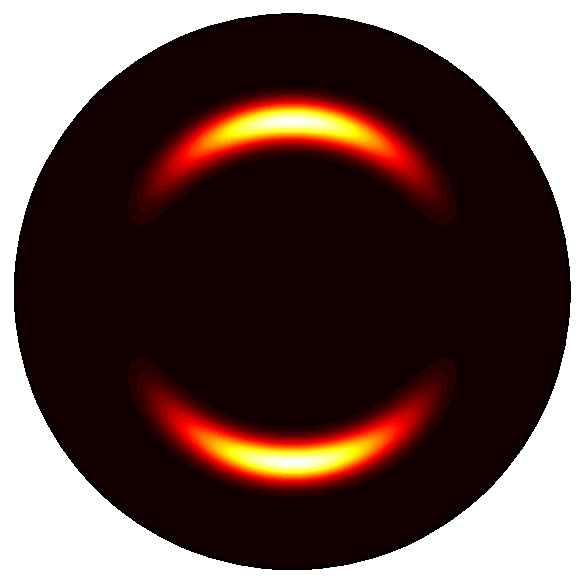
\includegraphics[width=\linewidth]{harmonic_iso_wave.pdf}
        \end{subfigure}
        \begin{subfigure}{.4\linewidth}
            \centering
            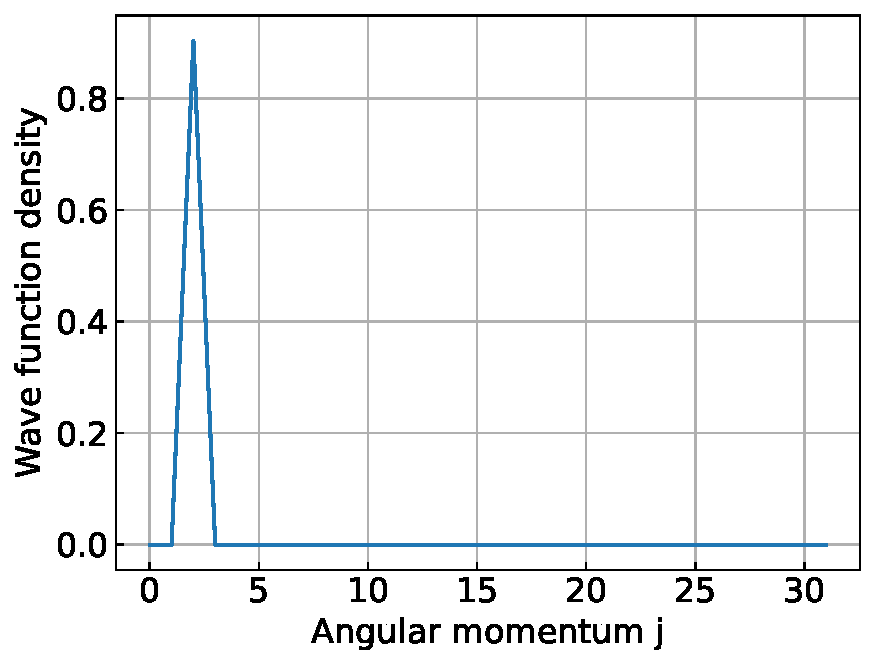
\includegraphics[width=\linewidth]{harmonic_iso_angular.pdf}
        \end{subfigure}
        \begin{subfigure}{.4\linewidth}
            \centering
            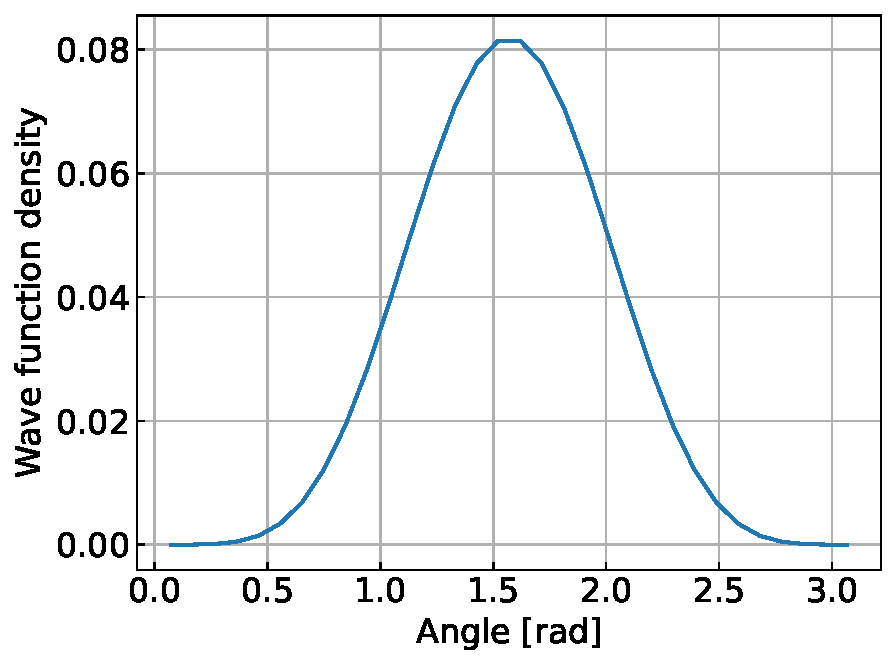
\includegraphics[width=\linewidth]{harmonic_iso_polar.pdf}
        \end{subfigure}
        \caption{Wave function densities for calculated ground state with $J = 2$ and without coriolis effect.}
    \end{figure}

    \begin{figure}[H]
        \centering
        \begin{subfigure}{.4\linewidth}
            \centering
            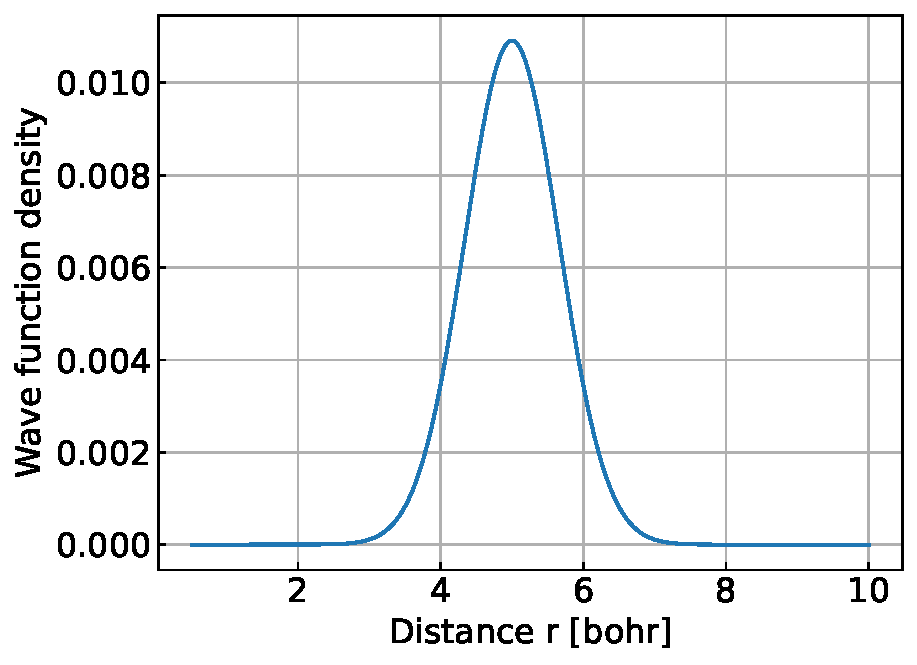
\includegraphics[width=\linewidth]{harmonic_iso_coriolis_distance.pdf}
        \end{subfigure}
        \begin{subfigure}{.4\linewidth}
            \centering
            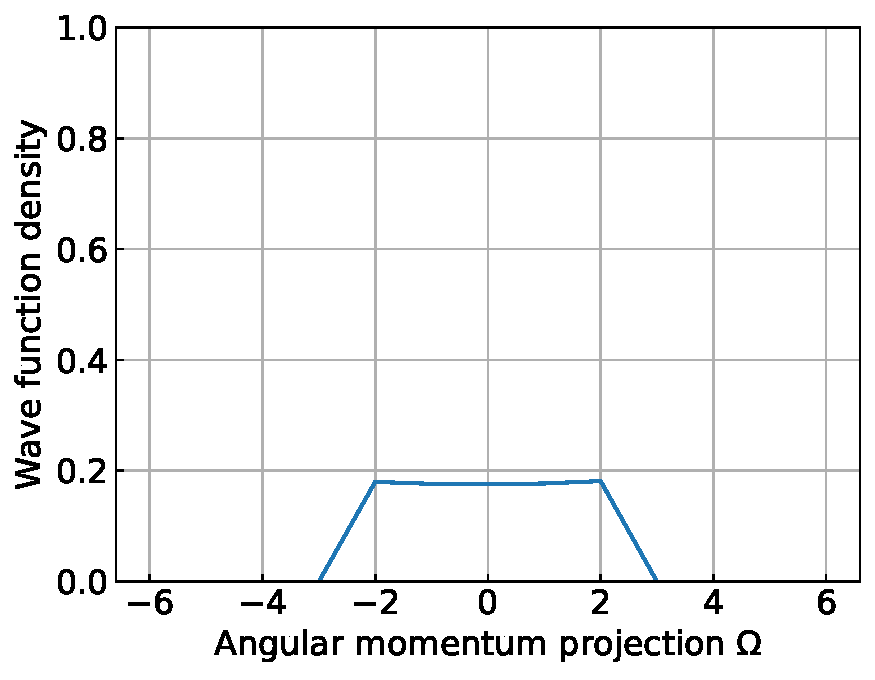
\includegraphics[width=\linewidth]{harmonic_iso_coriolis_omega.pdf}
        \end{subfigure}     
        \begin{subfigure}{.4\linewidth}
            \centering
            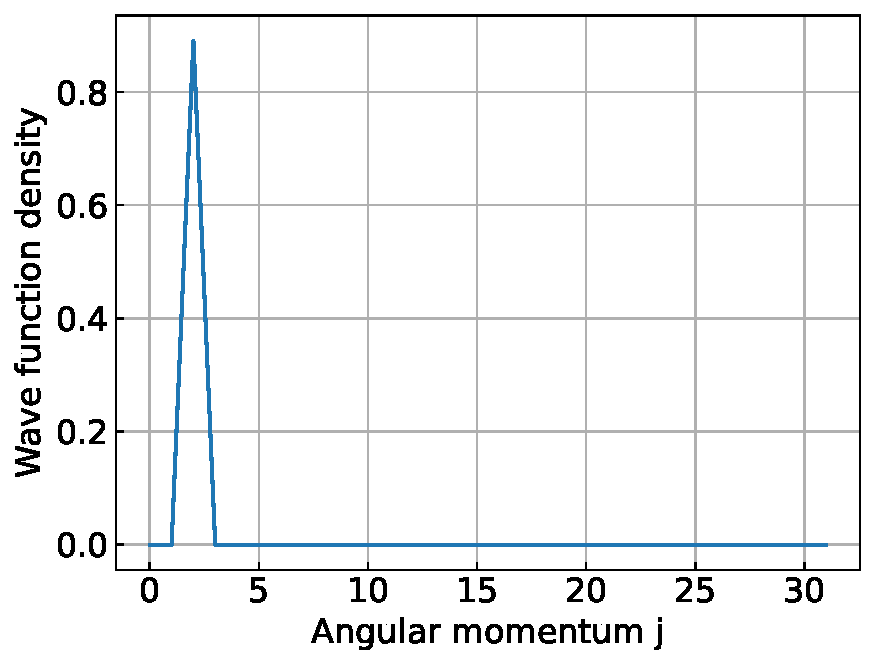
\includegraphics[width=\linewidth]{harmonic_iso_coriolis_angular.pdf}
        \end{subfigure}
        \begin{subfigure}{.4\linewidth}
            \centering
            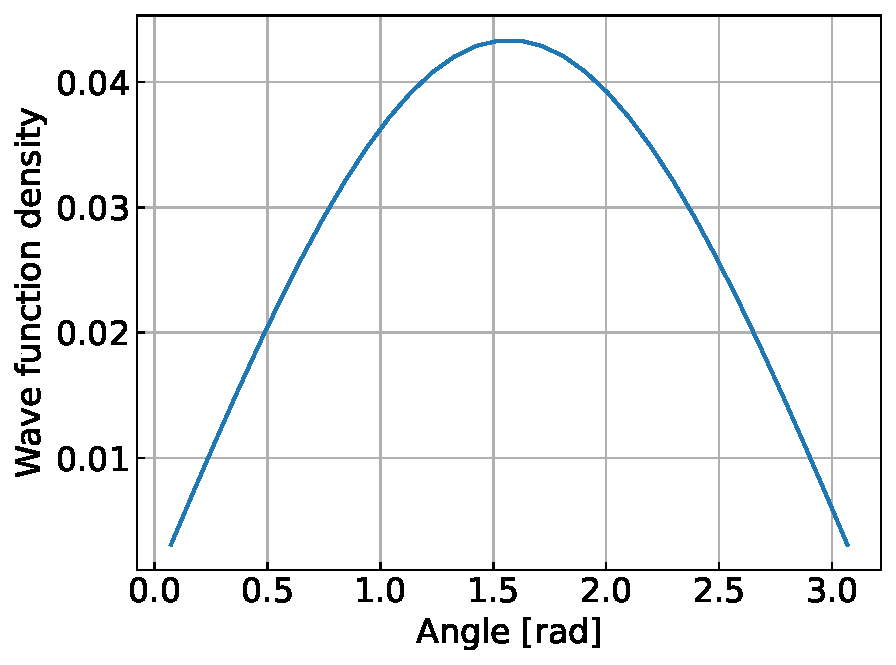
\includegraphics[width=\linewidth]{harmonic_iso_coriolis_polar.pdf}
        \end{subfigure}   
        \caption{Wave function densities for calculated ground state with $J = 2$ and coriolis effect.}
    \end{figure}

    For the potential of the form $V(r, \theta, \phi)$ the space-fixed Hamiltonian doesn't have any
    conserved angular numbers, however in the body-fixed frame we have still $J$ conserved.
    It can be deduced that in the case of $B = 0$, $J$ gives additional infinite degeneracy.
    Because of that, for every conserved $J$, the ground state is $\omega$, however it is only achievable
    with the inclusion of the coriolis effect.

    Additionally, we test the direct effect of the coriolis effect by multiplying
    the coriolis term by a factor, results are shown below.

    \begin{figure}[H]
        \centering
        \begin{subfigure}{.7\linewidth}
            \centering
            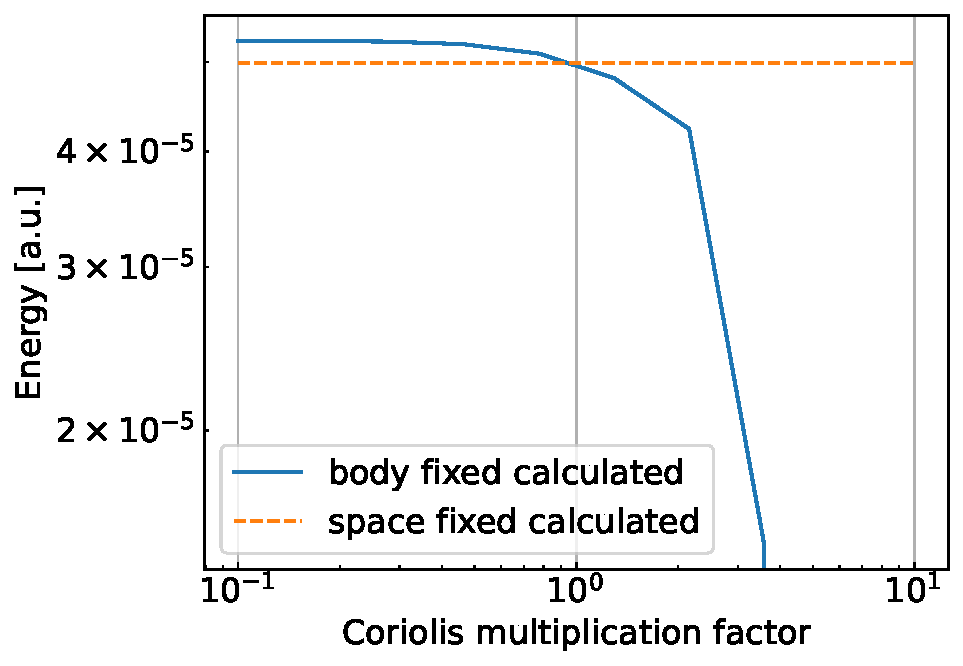
\includegraphics[width=\linewidth]{coriolis_convergence_test.pdf}
        \end{subfigure} 
        \caption{Calculated ground state energy dependence on the coriolis multiplication factor.}
    \end{figure}

\section{Reaction rate dependence on the coriolis effect body-fixed projection cutoff}
    Animations of collision with high $\Omega_\text{max}$ showed that the mixing of 
    the total projection is up to $\Omega = 45$. However reaction rate calculations converge 
    for $\Omega_\text{max} = 2$ as shown below, which means that mixing of $\Omega$ happens mostly after the collision.

    \begin{figure}[H]
        \centering
        \begin{subfigure}{.4\linewidth}
            \centering
            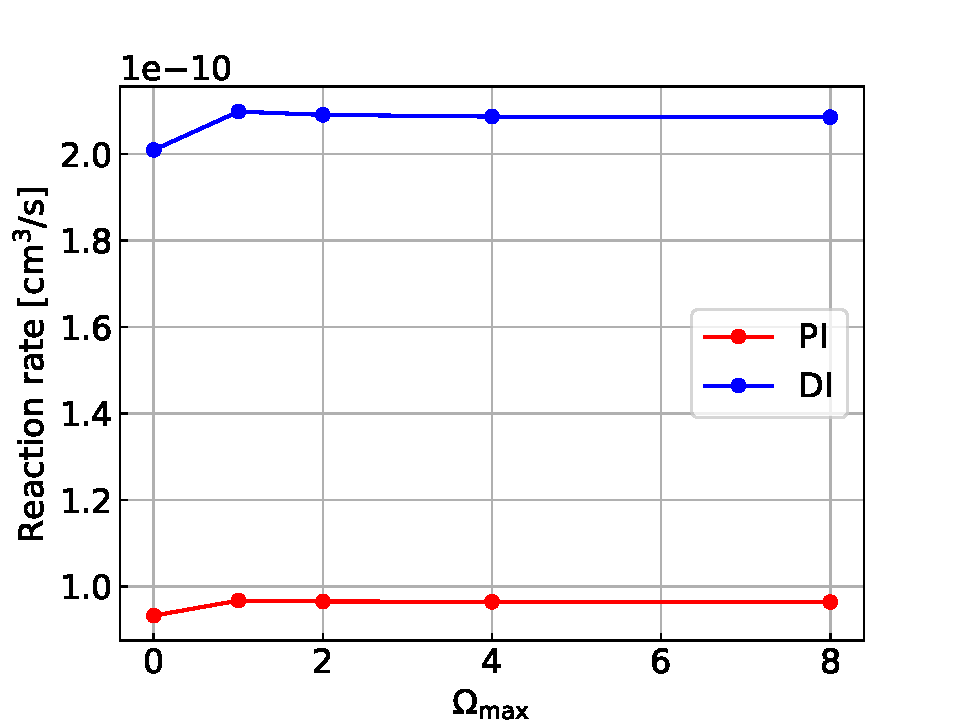
\includegraphics[width=\linewidth]{coriolis_rr_omega_maxes_0.pdf}
            \caption{Reaction rate for $j = 0$.}
        \end{subfigure}
        \begin{subfigure}{.4\linewidth}
            \centering
            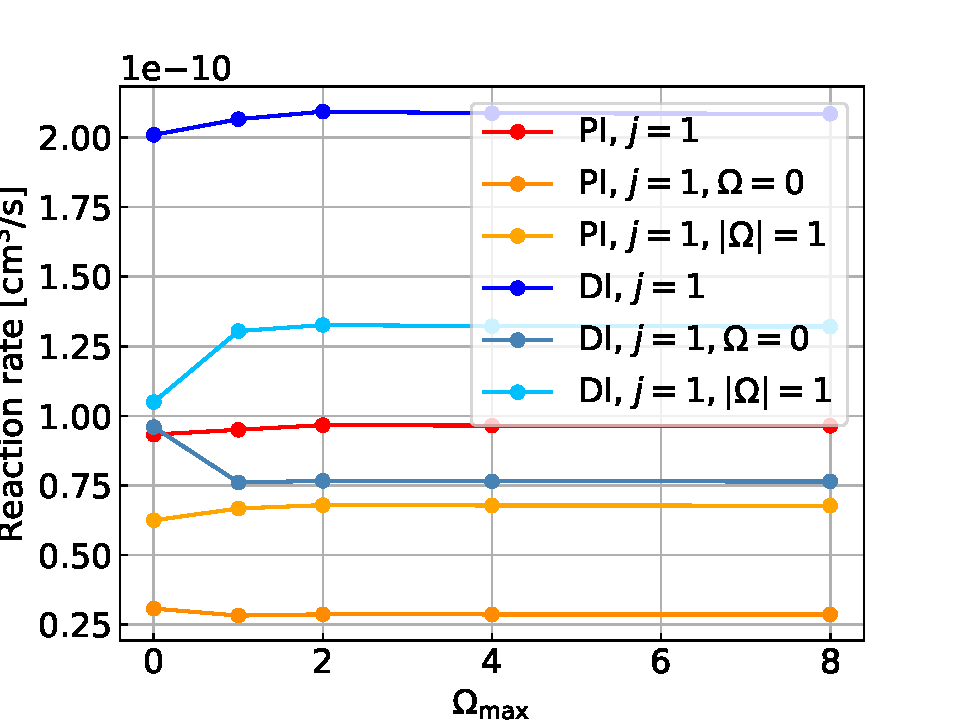
\includegraphics[width=\linewidth]{coriolis_rr_omega_maxes_1.pdf}
            \caption{Reaction rate for $j = 1$.}
        \end{subfigure}     
        \caption{Calculated reaction rates dependence on $\Omega_\text{max}$.}
    \end{figure}

    \begin{figure}[H]
        \centering
        \begin{subfigure}{.7\linewidth}
            \centering
            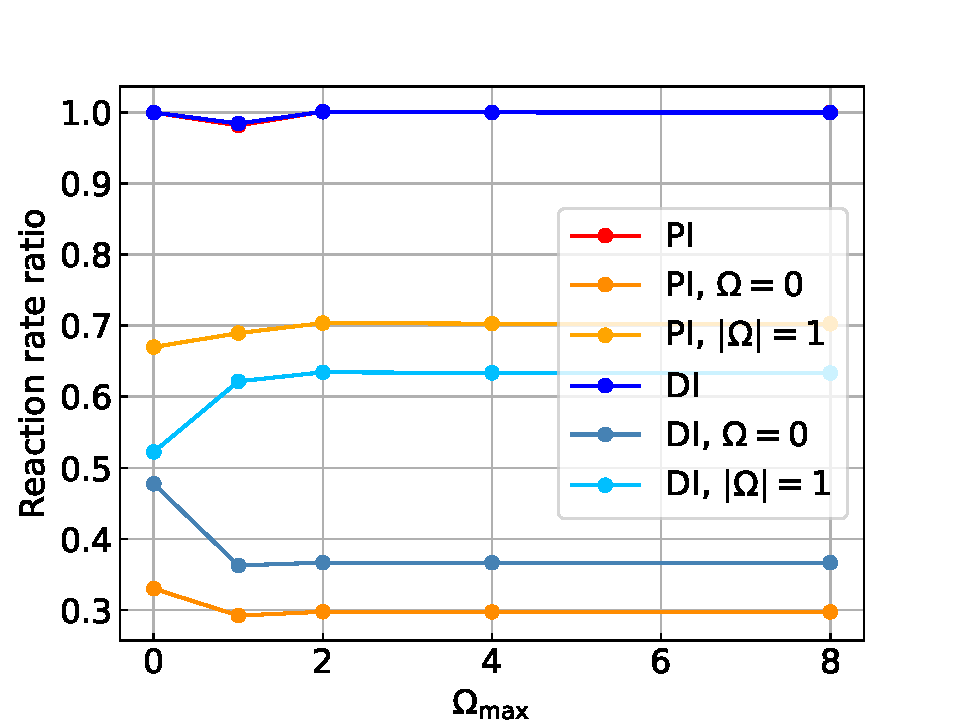
\includegraphics[width=\linewidth]{coriolis_rr_omega_maxes_ratio.pdf}
        \end{subfigure} 
        \caption{Calculated reaction rate ratio between $j = 1$ and $j = 0$, dependence on $\Omega_\text{max}$.}
    \end{figure}

\section{Reaction rate for superposition states}
    For the initial state $j = 1$ being the superposition of initial body-fixed projections
    \begin{equation}
        \ket{\psi} = \frac{1}{\sqrt{3}} \left(e^{i\phi_{-1}}\ket{-1} + \ket{0} + e^{\phi_1}\ket{1}\right),
    \end{equation}
    the reaction rate for different initial relative phases is shown below.

    \begin{figure}[H]
        \centering
        \begin{subfigure}{.4\linewidth}
            \centering
            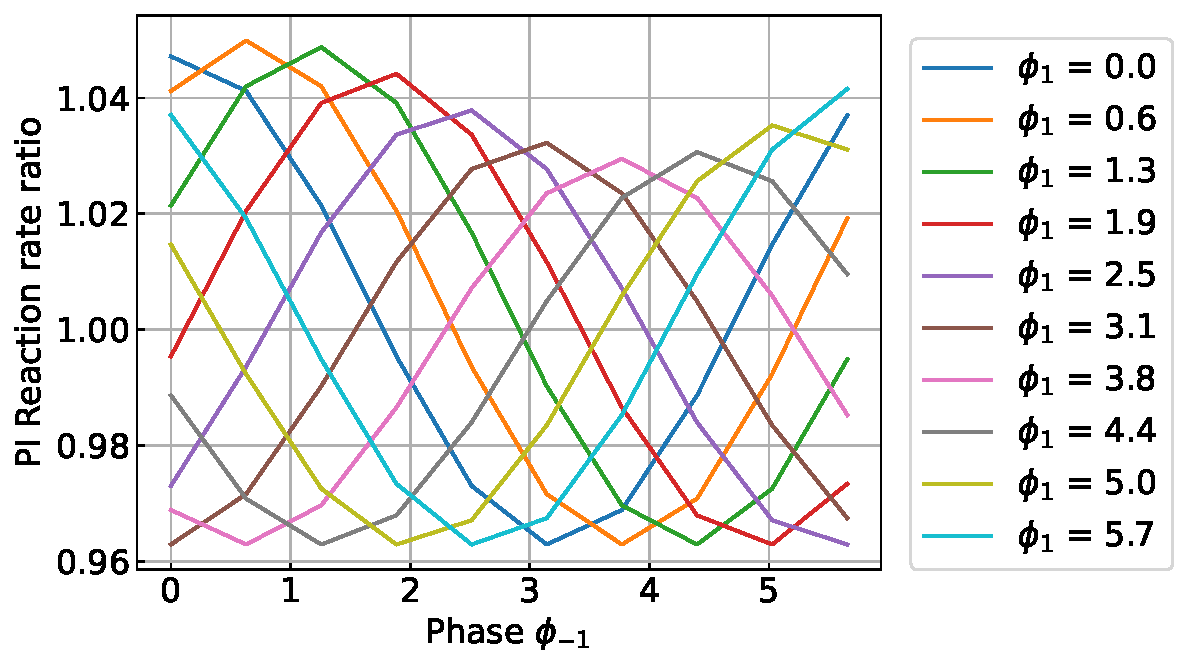
\includegraphics[width=\linewidth]{PI_reaction_ratio_phases.pdf}
            \caption{Penning ionization reaction rate ratios for different relative phases.}
        \end{subfigure}
        \begin{subfigure}{.4\linewidth}
            \centering
            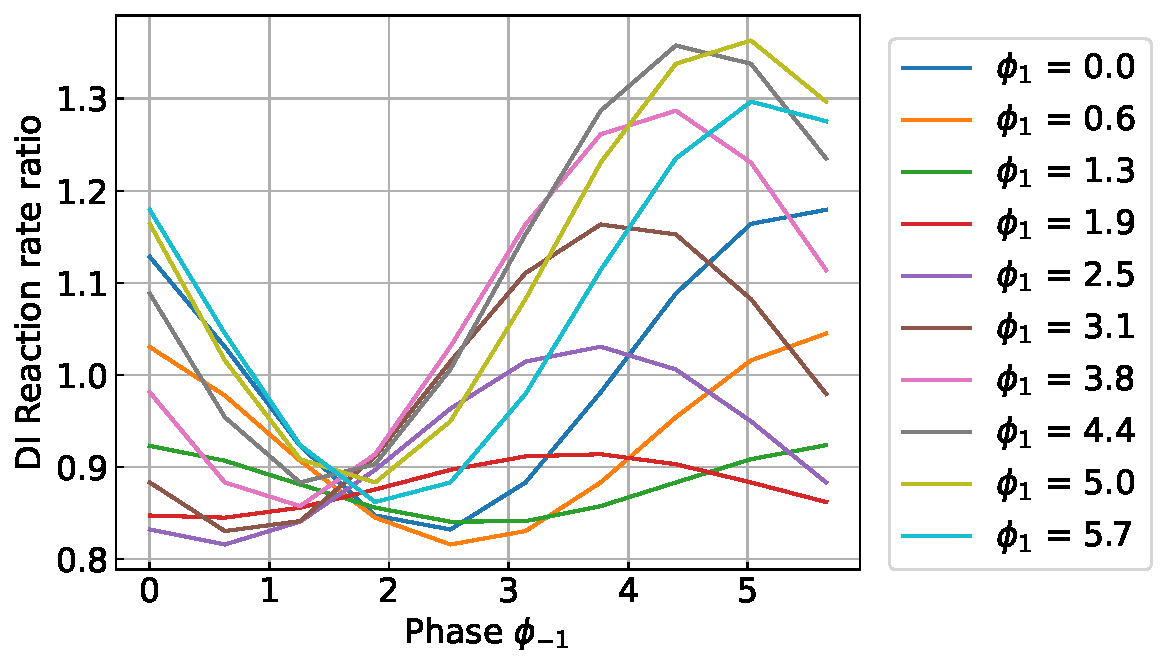
\includegraphics[width=\linewidth]{DI_reaction_ratio_phases.pdf}
            \caption{Dissociative ionization reaction rate ratios for different relative phases.}
        \end{subfigure}     
        \caption{Reaction rate ratios for different relative phases.}
    \end{figure}

    \begin{figure}[H]
        \centering
        \begin{subfigure}{.4\linewidth}
            \centering
            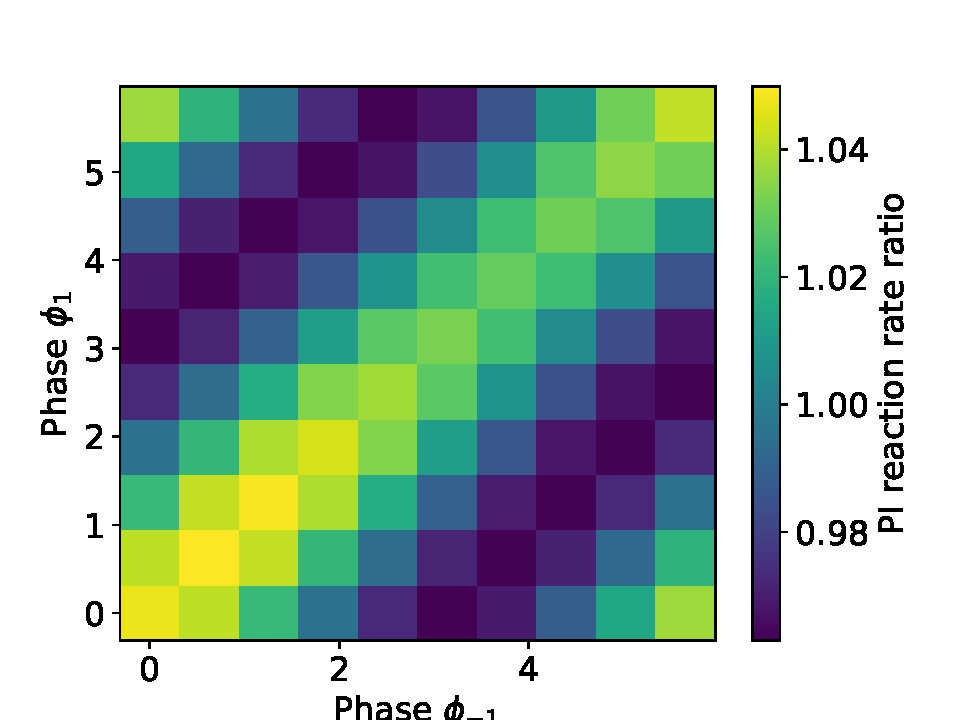
\includegraphics[width=\linewidth]{PI_reaction_ratio_phases_2d.pdf}
            \caption{Penning ionization reaction rate ratios for different relative phases.}
        \end{subfigure}
        \begin{subfigure}{.4\linewidth}
            \centering
            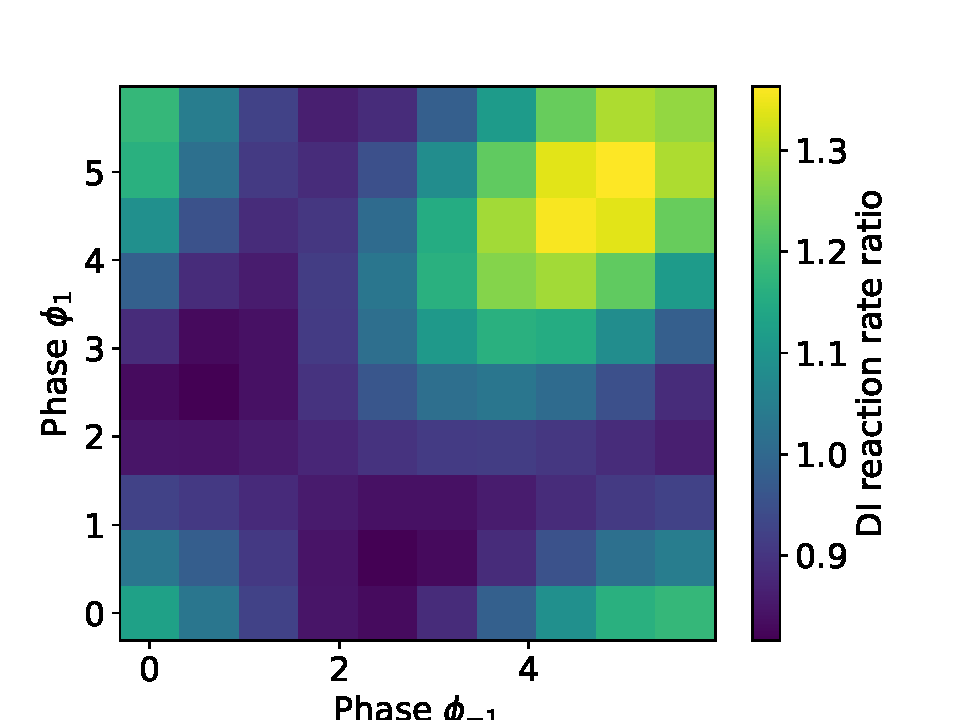
\includegraphics[width=\linewidth]{DI_reaction_ratio_phases_2d.pdf}
            \caption{Dissociative ionization reaction rate ratios for different relative phases.}
        \end{subfigure}     
        \caption{Reaction rate ratios for different relative phases.}
    \end{figure}
    Notice that the reaction rate ratio changes from 1 far more for DI channel than the PI channel, 
    which is consistent with the results of the experiment for which ratio for PI is much closer to 1 and DI is not.

    We additionally calculated, for every relative phases, the alignment evolution as shown below. 
    \begin{figure}[H]
        \centering
        \begin{subfigure}{.7\linewidth}
            \centering
            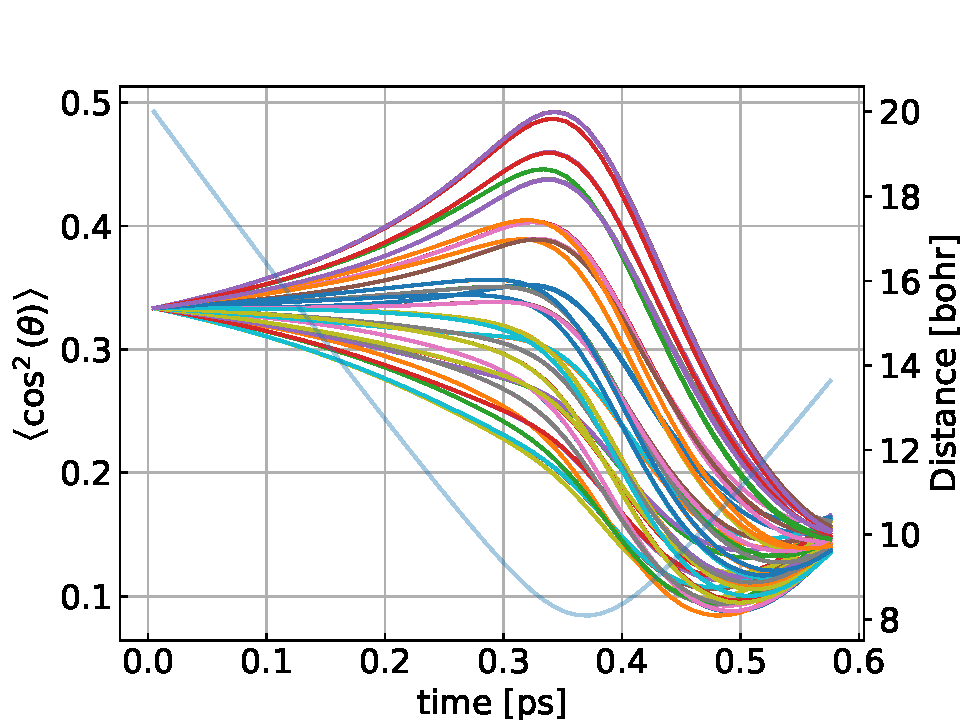
\includegraphics[width=\linewidth]{alignments_coriolis_phases.pdf}
        \end{subfigure} 
        \caption{Calculated alignments during the collision for different relative phases.}
    \end{figure}

    This brings the idea that after the OCS free flight there is a coherent relative phase in the case of $j = 1$,
    this relative coherence might be a result of the geometry of the experimental setup or various electric/magnetic fields.
\end{document}